% Created by tikzDevice version 0.12.3.1 on 2023-05-19 13:09:43
% !TEX encoding = UTF-8 Unicode
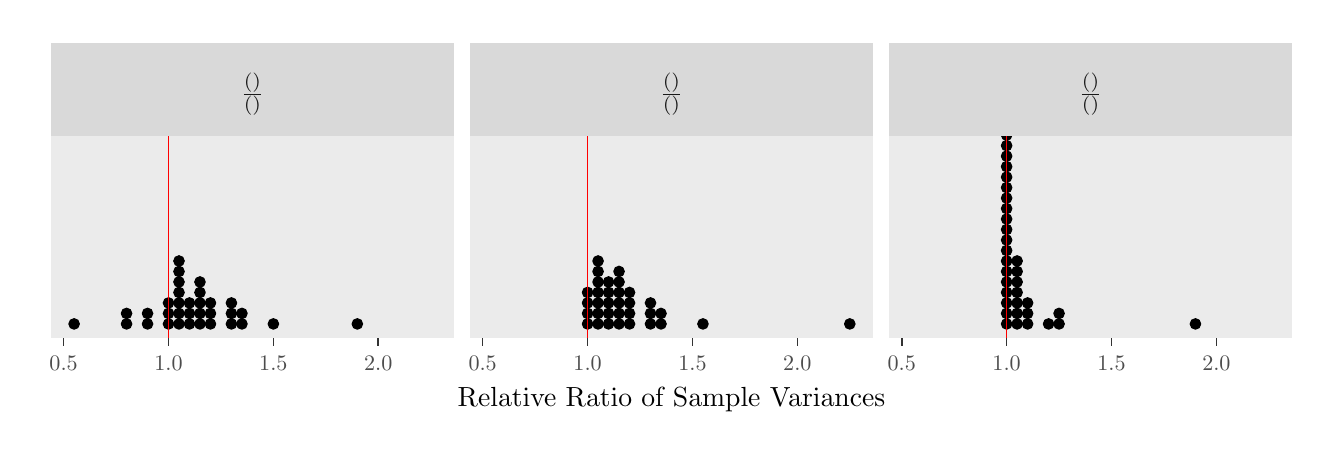
\begin{tikzpicture}[x=1pt,y=1pt]
\definecolor{fillColor}{RGB}{255,255,255}
\path[use as bounding box,fill=fillColor,fill opacity=0.00] (0,0) rectangle (462.53,144.54);
\begin{scope}
\path[clip] (  0.00,  0.00) rectangle (462.53,144.54);
\definecolor{drawColor}{RGB}{255,255,255}
\definecolor{fillColor}{RGB}{255,255,255}

\path[draw=drawColor,line width= 0.6pt,line join=round,line cap=round,fill=fillColor] (  0.00,  0.00) rectangle (462.53,144.54);
\end{scope}
\begin{scope}
\path[clip] (  8.25, 32.28) rectangle (154.18,105.24);
\definecolor{fillColor}{gray}{0.92}

\path[fill=fillColor] (  8.25, 32.28) rectangle (154.18,105.24);
\definecolor{drawColor}{RGB}{0,0,0}
\definecolor{fillColor}{RGB}{0,0,0}

\path[draw=drawColor,line width= 0.4pt,line join=round,fill=fillColor] ( 16.78, 37.49) circle (  1.90);

\path[draw=drawColor,line width= 0.4pt,line join=round,fill=fillColor] ( 35.73, 37.49) circle (  1.90);

\path[draw=drawColor,line width= 0.4pt,line join=round,fill=fillColor] ( 35.73, 41.28) circle (  1.90);

\path[draw=drawColor,line width= 0.4pt,line join=round,fill=fillColor] ( 43.31, 37.49) circle (  1.90);

\path[draw=drawColor,line width= 0.4pt,line join=round,fill=fillColor] ( 43.31, 41.28) circle (  1.90);

\path[draw=drawColor,line width= 0.4pt,line join=round,fill=fillColor] ( 50.89, 37.49) circle (  1.90);

\path[draw=drawColor,line width= 0.4pt,line join=round,fill=fillColor] ( 50.89, 41.28) circle (  1.90);

\path[draw=drawColor,line width= 0.4pt,line join=round,fill=fillColor] ( 50.89, 45.07) circle (  1.90);

\path[draw=drawColor,line width= 0.4pt,line join=round,fill=fillColor] ( 54.68, 37.49) circle (  1.90);

\path[draw=drawColor,line width= 0.4pt,line join=round,fill=fillColor] ( 54.68, 41.28) circle (  1.90);

\path[draw=drawColor,line width= 0.4pt,line join=round,fill=fillColor] ( 54.68, 45.07) circle (  1.90);

\path[draw=drawColor,line width= 0.4pt,line join=round,fill=fillColor] ( 54.68, 48.86) circle (  1.90);

\path[draw=drawColor,line width= 0.4pt,line join=round,fill=fillColor] ( 54.68, 52.65) circle (  1.90);

\path[draw=drawColor,line width= 0.4pt,line join=round,fill=fillColor] ( 54.68, 56.44) circle (  1.90);

\path[draw=drawColor,line width= 0.4pt,line join=round,fill=fillColor] ( 54.68, 60.23) circle (  1.90);

\path[draw=drawColor,line width= 0.4pt,line join=round,fill=fillColor] ( 58.47, 37.49) circle (  1.90);

\path[draw=drawColor,line width= 0.4pt,line join=round,fill=fillColor] ( 58.47, 41.28) circle (  1.90);

\path[draw=drawColor,line width= 0.4pt,line join=round,fill=fillColor] ( 58.47, 45.07) circle (  1.90);

\path[draw=drawColor,line width= 0.4pt,line join=round,fill=fillColor] ( 62.26, 37.49) circle (  1.90);

\path[draw=drawColor,line width= 0.4pt,line join=round,fill=fillColor] ( 62.26, 41.28) circle (  1.90);

\path[draw=drawColor,line width= 0.4pt,line join=round,fill=fillColor] ( 62.26, 45.07) circle (  1.90);

\path[draw=drawColor,line width= 0.4pt,line join=round,fill=fillColor] ( 62.26, 48.86) circle (  1.90);

\path[draw=drawColor,line width= 0.4pt,line join=round,fill=fillColor] ( 62.26, 52.65) circle (  1.90);

\path[draw=drawColor,line width= 0.4pt,line join=round,fill=fillColor] ( 66.05, 37.49) circle (  1.90);

\path[draw=drawColor,line width= 0.4pt,line join=round,fill=fillColor] ( 66.05, 41.28) circle (  1.90);

\path[draw=drawColor,line width= 0.4pt,line join=round,fill=fillColor] ( 66.05, 45.07) circle (  1.90);

\path[draw=drawColor,line width= 0.4pt,line join=round,fill=fillColor] ( 73.63, 37.49) circle (  1.90);

\path[draw=drawColor,line width= 0.4pt,line join=round,fill=fillColor] ( 73.63, 41.28) circle (  1.90);

\path[draw=drawColor,line width= 0.4pt,line join=round,fill=fillColor] ( 73.63, 45.07) circle (  1.90);

\path[draw=drawColor,line width= 0.4pt,line join=round,fill=fillColor] ( 77.42, 37.49) circle (  1.90);

\path[draw=drawColor,line width= 0.4pt,line join=round,fill=fillColor] ( 77.42, 41.28) circle (  1.90);

\path[draw=drawColor,line width= 0.4pt,line join=round,fill=fillColor] ( 88.79, 37.49) circle (  1.90);

\path[draw=drawColor,line width= 0.4pt,line join=round,fill=fillColor] (119.12, 37.49) circle (  1.90);
\definecolor{drawColor}{RGB}{255,0,0}

\path[draw=drawColor,line width= 0.6pt,line join=round] ( 50.89, 32.28) -- ( 50.89,105.24);
\end{scope}
\begin{scope}
\path[clip] (159.68, 32.28) rectangle (305.60,105.24);
\definecolor{fillColor}{gray}{0.92}

\path[fill=fillColor] (159.68, 32.28) rectangle (305.60,105.24);
\definecolor{drawColor}{RGB}{0,0,0}
\definecolor{fillColor}{RGB}{0,0,0}

\path[draw=drawColor,line width= 0.4pt,line join=round,fill=fillColor] (202.32, 37.49) circle (  1.90);

\path[draw=drawColor,line width= 0.4pt,line join=round,fill=fillColor] (202.32, 41.28) circle (  1.90);

\path[draw=drawColor,line width= 0.4pt,line join=round,fill=fillColor] (202.32, 45.07) circle (  1.90);

\path[draw=drawColor,line width= 0.4pt,line join=round,fill=fillColor] (202.32, 48.86) circle (  1.90);

\path[draw=drawColor,line width= 0.4pt,line join=round,fill=fillColor] (206.11, 37.49) circle (  1.90);

\path[draw=drawColor,line width= 0.4pt,line join=round,fill=fillColor] (206.11, 41.28) circle (  1.90);

\path[draw=drawColor,line width= 0.4pt,line join=round,fill=fillColor] (206.11, 45.07) circle (  1.90);

\path[draw=drawColor,line width= 0.4pt,line join=round,fill=fillColor] (206.11, 48.86) circle (  1.90);

\path[draw=drawColor,line width= 0.4pt,line join=round,fill=fillColor] (206.11, 52.65) circle (  1.90);

\path[draw=drawColor,line width= 0.4pt,line join=round,fill=fillColor] (206.11, 56.44) circle (  1.90);

\path[draw=drawColor,line width= 0.4pt,line join=round,fill=fillColor] (206.11, 60.23) circle (  1.90);

\path[draw=drawColor,line width= 0.4pt,line join=round,fill=fillColor] (209.90, 37.49) circle (  1.90);

\path[draw=drawColor,line width= 0.4pt,line join=round,fill=fillColor] (209.90, 41.28) circle (  1.90);

\path[draw=drawColor,line width= 0.4pt,line join=round,fill=fillColor] (209.90, 45.07) circle (  1.90);

\path[draw=drawColor,line width= 0.4pt,line join=round,fill=fillColor] (209.90, 48.86) circle (  1.90);

\path[draw=drawColor,line width= 0.4pt,line join=round,fill=fillColor] (209.90, 52.65) circle (  1.90);

\path[draw=drawColor,line width= 0.4pt,line join=round,fill=fillColor] (213.69, 37.49) circle (  1.90);

\path[draw=drawColor,line width= 0.4pt,line join=round,fill=fillColor] (213.69, 41.28) circle (  1.90);

\path[draw=drawColor,line width= 0.4pt,line join=round,fill=fillColor] (213.69, 45.07) circle (  1.90);

\path[draw=drawColor,line width= 0.4pt,line join=round,fill=fillColor] (213.69, 48.86) circle (  1.90);

\path[draw=drawColor,line width= 0.4pt,line join=round,fill=fillColor] (213.69, 52.65) circle (  1.90);

\path[draw=drawColor,line width= 0.4pt,line join=round,fill=fillColor] (213.69, 56.44) circle (  1.90);

\path[draw=drawColor,line width= 0.4pt,line join=round,fill=fillColor] (217.48, 37.49) circle (  1.90);

\path[draw=drawColor,line width= 0.4pt,line join=round,fill=fillColor] (217.48, 41.28) circle (  1.90);

\path[draw=drawColor,line width= 0.4pt,line join=round,fill=fillColor] (217.48, 45.07) circle (  1.90);

\path[draw=drawColor,line width= 0.4pt,line join=round,fill=fillColor] (217.48, 48.86) circle (  1.90);

\path[draw=drawColor,line width= 0.4pt,line join=round,fill=fillColor] (225.06, 37.49) circle (  1.90);

\path[draw=drawColor,line width= 0.4pt,line join=round,fill=fillColor] (225.06, 41.28) circle (  1.90);

\path[draw=drawColor,line width= 0.4pt,line join=round,fill=fillColor] (225.06, 45.07) circle (  1.90);

\path[draw=drawColor,line width= 0.4pt,line join=round,fill=fillColor] (228.85, 37.49) circle (  1.90);

\path[draw=drawColor,line width= 0.4pt,line join=round,fill=fillColor] (228.85, 41.28) circle (  1.90);

\path[draw=drawColor,line width= 0.4pt,line join=round,fill=fillColor] (244.01, 37.49) circle (  1.90);

\path[draw=drawColor,line width= 0.4pt,line join=round,fill=fillColor] (297.07, 37.49) circle (  1.90);
\definecolor{drawColor}{RGB}{255,0,0}

\path[draw=drawColor,line width= 0.6pt,line join=round] (202.32, 32.28) -- (202.32,105.24);
\end{scope}
\begin{scope}
\path[clip] (311.10, 32.28) rectangle (457.03,105.24);
\definecolor{fillColor}{gray}{0.92}

\path[fill=fillColor] (311.10, 32.28) rectangle (457.03,105.24);
\definecolor{drawColor}{RGB}{0,0,0}
\definecolor{fillColor}{RGB}{0,0,0}

\path[draw=drawColor,line width= 0.4pt,line join=round,fill=fillColor] (353.74, 37.49) circle (  1.90);

\path[draw=drawColor,line width= 0.4pt,line join=round,fill=fillColor] (353.74, 41.28) circle (  1.90);

\path[draw=drawColor,line width= 0.4pt,line join=round,fill=fillColor] (353.74, 45.07) circle (  1.90);

\path[draw=drawColor,line width= 0.4pt,line join=round,fill=fillColor] (353.74, 48.86) circle (  1.90);

\path[draw=drawColor,line width= 0.4pt,line join=round,fill=fillColor] (353.74, 52.65) circle (  1.90);

\path[draw=drawColor,line width= 0.4pt,line join=round,fill=fillColor] (353.74, 56.44) circle (  1.90);

\path[draw=drawColor,line width= 0.4pt,line join=round,fill=fillColor] (353.74, 60.23) circle (  1.90);

\path[draw=drawColor,line width= 0.4pt,line join=round,fill=fillColor] (353.74, 64.02) circle (  1.90);

\path[draw=drawColor,line width= 0.4pt,line join=round,fill=fillColor] (353.74, 67.81) circle (  1.90);

\path[draw=drawColor,line width= 0.4pt,line join=round,fill=fillColor] (353.74, 71.60) circle (  1.90);

\path[draw=drawColor,line width= 0.4pt,line join=round,fill=fillColor] (353.74, 75.39) circle (  1.90);

\path[draw=drawColor,line width= 0.4pt,line join=round,fill=fillColor] (353.74, 79.18) circle (  1.90);

\path[draw=drawColor,line width= 0.4pt,line join=round,fill=fillColor] (353.74, 82.97) circle (  1.90);

\path[draw=drawColor,line width= 0.4pt,line join=round,fill=fillColor] (353.74, 86.76) circle (  1.90);

\path[draw=drawColor,line width= 0.4pt,line join=round,fill=fillColor] (353.74, 90.55) circle (  1.90);

\path[draw=drawColor,line width= 0.4pt,line join=round,fill=fillColor] (353.74, 94.34) circle (  1.90);

\path[draw=drawColor,line width= 0.4pt,line join=round,fill=fillColor] (353.74, 98.13) circle (  1.90);

\path[draw=drawColor,line width= 0.4pt,line join=round,fill=fillColor] (353.74,101.92) circle (  1.90);

\path[draw=drawColor,line width= 0.4pt,line join=round,fill=fillColor] (353.74,105.71) circle (  1.90);

\path[draw=drawColor,line width= 0.4pt,line join=round,fill=fillColor] (357.53, 37.49) circle (  1.90);

\path[draw=drawColor,line width= 0.4pt,line join=round,fill=fillColor] (357.53, 41.28) circle (  1.90);

\path[draw=drawColor,line width= 0.4pt,line join=round,fill=fillColor] (357.53, 45.07) circle (  1.90);

\path[draw=drawColor,line width= 0.4pt,line join=round,fill=fillColor] (357.53, 48.86) circle (  1.90);

\path[draw=drawColor,line width= 0.4pt,line join=round,fill=fillColor] (357.53, 52.65) circle (  1.90);

\path[draw=drawColor,line width= 0.4pt,line join=round,fill=fillColor] (357.53, 56.44) circle (  1.90);

\path[draw=drawColor,line width= 0.4pt,line join=round,fill=fillColor] (357.53, 60.23) circle (  1.90);

\path[draw=drawColor,line width= 0.4pt,line join=round,fill=fillColor] (361.32, 37.49) circle (  1.90);

\path[draw=drawColor,line width= 0.4pt,line join=round,fill=fillColor] (361.32, 41.28) circle (  1.90);

\path[draw=drawColor,line width= 0.4pt,line join=round,fill=fillColor] (361.32, 45.07) circle (  1.90);

\path[draw=drawColor,line width= 0.4pt,line join=round,fill=fillColor] (368.90, 37.49) circle (  1.90);

\path[draw=drawColor,line width= 0.4pt,line join=round,fill=fillColor] (372.69, 37.49) circle (  1.90);

\path[draw=drawColor,line width= 0.4pt,line join=round,fill=fillColor] (372.69, 41.28) circle (  1.90);

\path[draw=drawColor,line width= 0.4pt,line join=round,fill=fillColor] (421.97, 37.49) circle (  1.90);
\definecolor{drawColor}{RGB}{255,0,0}

\path[draw=drawColor,line width= 0.6pt,line join=round] (353.74, 32.28) -- (353.74,105.24);
\end{scope}
\begin{scope}
\path[clip] (  8.25,105.24) rectangle (154.18,139.04);
\definecolor{fillColor}{gray}{0.85}

\path[fill=fillColor] (  8.25,105.24) rectangle (154.18,139.04);
\definecolor{drawColor}{gray}{0.10}

\node[text=drawColor,anchor=base,inner sep=0pt, outer sep=0pt, scale=  1.00] at ( 81.21,125.21) {};

\node[text=drawColor,anchor=base,inner sep=0pt, outer sep=0pt, scale=  1.00] at ( 81.21,118.01) {$\frac{\varhat(\tsd)}{\varhat(\trebar)}$};

\node[text=drawColor,anchor=base,inner sep=0pt, outer sep=0pt, scale=  1.00] at ( 81.21,110.81) {};
\end{scope}
\begin{scope}
\path[clip] (159.68,105.24) rectangle (305.60,139.04);
\definecolor{fillColor}{gray}{0.85}

\path[fill=fillColor] (159.68,105.24) rectangle (305.60,139.04);
\definecolor{drawColor}{gray}{0.10}

\node[text=drawColor,anchor=base,inner sep=0pt, outer sep=0pt, scale=  1.00] at (232.64,125.21) {};

\node[text=drawColor,anchor=base,inner sep=0pt, outer sep=0pt, scale=  1.00] at (232.64,118.01) {$\frac{\varhat(\tsd)}{\varhat(\trc)}$};

\node[text=drawColor,anchor=base,inner sep=0pt, outer sep=0pt, scale=  1.00] at (232.64,110.81) {};
\end{scope}
\begin{scope}
\path[clip] (311.10,105.24) rectangle (457.03,139.04);
\definecolor{fillColor}{gray}{0.85}

\path[fill=fillColor] (311.10,105.24) rectangle (457.03,139.04);
\definecolor{drawColor}{gray}{0.10}

\node[text=drawColor,anchor=base,inner sep=0pt, outer sep=0pt, scale=  1.00] at (384.06,125.21) {};

\node[text=drawColor,anchor=base,inner sep=0pt, outer sep=0pt, scale=  1.00] at (384.06,118.01) {$\frac{\varhat(\trebar)}{\varhat(\trc)}$};

\node[text=drawColor,anchor=base,inner sep=0pt, outer sep=0pt, scale=  1.00] at (384.06,110.81) {};
\end{scope}
\begin{scope}
\path[clip] (  0.00,  0.00) rectangle (462.53,144.54);
\definecolor{drawColor}{gray}{0.20}

\path[draw=drawColor,line width= 0.6pt,line join=round] ( 12.99, 29.53) --
	( 12.99, 32.28);

\path[draw=drawColor,line width= 0.6pt,line join=round] ( 50.89, 29.53) --
	( 50.89, 32.28);

\path[draw=drawColor,line width= 0.6pt,line join=round] ( 88.79, 29.53) --
	( 88.79, 32.28);

\path[draw=drawColor,line width= 0.6pt,line join=round] (126.70, 29.53) --
	(126.70, 32.28);
\end{scope}
\begin{scope}
\path[clip] (  0.00,  0.00) rectangle (462.53,144.54);
\definecolor{drawColor}{gray}{0.30}

\node[text=drawColor,anchor=base,inner sep=0pt, outer sep=0pt, scale=  0.80] at ( 12.99, 20.71) {0.5};

\node[text=drawColor,anchor=base,inner sep=0pt, outer sep=0pt, scale=  0.80] at ( 50.89, 20.71) {1.0};

\node[text=drawColor,anchor=base,inner sep=0pt, outer sep=0pt, scale=  0.80] at ( 88.79, 20.71) {1.5};

\node[text=drawColor,anchor=base,inner sep=0pt, outer sep=0pt, scale=  0.80] at (126.70, 20.71) {2.0};
\end{scope}
\begin{scope}
\path[clip] (  0.00,  0.00) rectangle (462.53,144.54);
\definecolor{drawColor}{gray}{0.20}

\path[draw=drawColor,line width= 0.6pt,line join=round] (164.41, 29.53) --
	(164.41, 32.28);

\path[draw=drawColor,line width= 0.6pt,line join=round] (202.32, 29.53) --
	(202.32, 32.28);

\path[draw=drawColor,line width= 0.6pt,line join=round] (240.22, 29.53) --
	(240.22, 32.28);

\path[draw=drawColor,line width= 0.6pt,line join=round] (278.12, 29.53) --
	(278.12, 32.28);
\end{scope}
\begin{scope}
\path[clip] (  0.00,  0.00) rectangle (462.53,144.54);
\definecolor{drawColor}{gray}{0.30}

\node[text=drawColor,anchor=base,inner sep=0pt, outer sep=0pt, scale=  0.80] at (164.41, 20.71) {0.5};

\node[text=drawColor,anchor=base,inner sep=0pt, outer sep=0pt, scale=  0.80] at (202.32, 20.71) {1.0};

\node[text=drawColor,anchor=base,inner sep=0pt, outer sep=0pt, scale=  0.80] at (240.22, 20.71) {1.5};

\node[text=drawColor,anchor=base,inner sep=0pt, outer sep=0pt, scale=  0.80] at (278.12, 20.71) {2.0};
\end{scope}
\begin{scope}
\path[clip] (  0.00,  0.00) rectangle (462.53,144.54);
\definecolor{drawColor}{gray}{0.20}

\path[draw=drawColor,line width= 0.6pt,line join=round] (315.84, 29.53) --
	(315.84, 32.28);

\path[draw=drawColor,line width= 0.6pt,line join=round] (353.74, 29.53) --
	(353.74, 32.28);

\path[draw=drawColor,line width= 0.6pt,line join=round] (391.65, 29.53) --
	(391.65, 32.28);

\path[draw=drawColor,line width= 0.6pt,line join=round] (429.55, 29.53) --
	(429.55, 32.28);
\end{scope}
\begin{scope}
\path[clip] (  0.00,  0.00) rectangle (462.53,144.54);
\definecolor{drawColor}{gray}{0.30}

\node[text=drawColor,anchor=base,inner sep=0pt, outer sep=0pt, scale=  0.80] at (315.84, 20.71) {0.5};

\node[text=drawColor,anchor=base,inner sep=0pt, outer sep=0pt, scale=  0.80] at (353.74, 20.71) {1.0};

\node[text=drawColor,anchor=base,inner sep=0pt, outer sep=0pt, scale=  0.80] at (391.65, 20.71) {1.5};

\node[text=drawColor,anchor=base,inner sep=0pt, outer sep=0pt, scale=  0.80] at (429.55, 20.71) {2.0};
\end{scope}
\begin{scope}
\path[clip] (  0.00,  0.00) rectangle (462.53,144.54);
\definecolor{drawColor}{RGB}{0,0,0}

\node[text=drawColor,anchor=base,inner sep=0pt, outer sep=0pt, scale=  1.00] at (232.64,  7.83) {Relative Ratio of Sample Variances};
\end{scope}
\end{tikzpicture}
